\chapter{General discussion and recommendations}
\section{Introduction}

The principal objective of this thesis has been to characterise
the Galician shelf response to the varying seasonal forcing, in
particular to identify the typical spatial variability of wind and
its effect on the shelf circulation. Through a set of observations
including satellite data (scatterometer, AVHRR, SeaWIFS and
drifters), cruise data (CTD, ADCP, turbulence probe) and mooring
data (wind and surface currents) the complex shelf circulation and
its response to large scale forcing has been explored. Many of the
observations, although limited in their spatial and temporal
coverage, are novel in an area where systematic sampling has been
sparse. In chapter~\ref{ch:winds}, for the first time, the spatial
and highly temporal variability of the wind has been unequivocally
shown and indirect evidence of its effect, through SST has been
presented. Results from Chapter~\ref{ch:winds} were extrapolated
to help the interpretation of SST data in the absence of direct
spatial wind measurements. In subsequent chapters, examples of the
spring transition, upwelling season and autumn
transition/downwelling stage have been presented covering the
contrasting shelf environments identified for the Galician CTZ in
the literature. The last chapter provided an integrated
quantitative view of the Lagrangian differences between the
upwelling and downwelling regime.

\section{Shelf classification} The gently sloping shelf around
Galicia extends, on average, 40km seawards either side of Cape
Finisterre (with a minimum at the Cape of 20km) constituting a
long narrow shelf.  Even in the absence of filament formation, the
upwelling front extends beyond the shelf break into waters
$>$1000m. This is expected during sustained favourable upwelling
winds, as happens in central California \citep{Brink83}, or for a
narrow shelf, as in Galicia. The front's offshore position is an
indication of weak topographic control, in contrast with the
stronger link reported by \citet{Fiuza96b} and \citet{Peliz02} in
the wider Portuguese shelf south of 41\deg
(Figs~\ref{fig:largebathy} and~\ref{fig:summerupw}c). The poleward
undercurrent is located off-shelf during strong upwelling wind
episodes (Chapters~\ref{ch:spring}-\ref{ch:cd114}) and the shelf
can be expected to function like a shallow one, with surface and
bottom Ekman layers occupying the entire water column in a two
layer circulation \citep{Hill98}. It is only during wind
relaxations (Chapter\ref{ch:cd114}) that the poleward undercurrent
occupies the shelf.

The small width of the shelf means there is a strong interaction
between the shelf circulation, the circulation inside the Rias and
the wind forcing. Previous authors have acknowledged this for the
Rias Bajas \citep[e.g.][]{Gomez-Gesteira01,Prego01,Sordo01} and
they have to be considered an integral part of the shelf in as
much as it responds to the same forcings.



\section{Variability} It has been shown that the upwelling region
of Galicia is a highly variable system. Two main interconnected
sources of variability have been identified in the present work:
the irregular coastline and shelf with its major example in Cape
Finisterre, and the strong variability at spatial and temporal
scales of the wind forcing. Both aspects affect the development
and evolution of the upwelling regime (Chapter~\ref{ch:winds})
\citep[e.g.][]{Barth00,Samelson02} and the downwelling regime
\citep[e.g.][]{Dubert98}. Small Time scales have been consistently
obtained from Lagrangian observations and large scale winds and
hint at a very dynamic region. Despite its complexity, the
mesoscale wind variability can be reduced to a finite number of
spatial patterns which, to a first approximation, explain the
Galician shelf response (Chapter~\ref{ch:winds}). One quarter of
the wind spatial variability rests in increasingly complex spatial
patterns, while three quarters correspond to a coherent wind. The
seasonality of the wind forcing is masked by upwelling/downwelling
patterns throughout the year. However, the system response shows a
clearer seasonality with upwelling during the summer and
downwelling during winter mediated by a meridional density
gradient. It is the more consistent upwelling winds during the
summer that determine this seasonality. However, the intermittent
winds (Time scales of 2-3 days, Chapter~\ref{ch:winds}) produce a
complex contouring front with a broad upwelling front
(Chapter~\ref{ch:cd114}, Fig~\ref{fig:cd114_shelftran}) rather
than the sharp one measured south in the broader Portuguese shelf
\citep{Peliz02}. Further south, along the Portuguese coast, the
wind is expected to be less variable  similarly to
Oregon-California differences. Nonetheless, interannual
differences in the upwelling and downwelling regimes are large
\citep{Huthnance02} and related to the wind. Unusual predominance
of PUNC over PUWC patterns restrict filament development on the
west coast while enhancing the Cape Finisterre filament as was the
case in 1999 (Chapter~\ref{ch:winds}). Integrated values of
monthly upwelling indices for the west coast (Vigo region, as in
Chapter~\ref{ch:cd105}) showed smaller values in 1999 (119)
compared to 1998 (273) when west coast filaments fully developed
(Chapter~\ref{ch:cd114}), which agrees with the expected
differences between ``PUNC'' and ``PUWC'' years. Similarly,
predominance of PUWC patterns over DOWN patterns during the winter
of 1999 precluded the development of the poleward flow over the
slope (Chapter~\ref{ch:drifters}).

With no clear seasonal wind changes in the scatterometer data the
transitional periods between downwelling and upwelling regimes are
difficult to examine. Monthly upwelling index
(Chapter~\ref{ch:cd114} suggest a mean long spring transition
(April to June) from the downwelling to upwelling regime for the
1986-1998 record, due to high wind variability. During those
months, co-existence of the PCC and coastal upwelling is possible
(Chapter~\ref{ch:spring}). However, upwelling relaxations or
downwelling winds quickly suppress the coastal upwelling (e.g.
Chapter~\ref{ch:winds}). The PCC was still present in June 1997
prior to the onset of coastal upwelling (Chapter~\ref{ch:spring}).
At this late stage, the PCC was better established offshore than
on the slope, where traces of it were scattered along the slope
but with no velocity signal. Differences with the PCC at the start
of the downwelling regime were large. No evidences were found of
an offshore PCC branch were found in October-November 1999.

\section{Seasonality} An schematic of the expected upper layer seasonal
circulation in the Galician shelf can be seen in
Fig~\ref{fig:concl_sketch}. THESE WILL NEED EXTENDING (SORRY I
COULDN'T MANAGE TO FINISH IT!)

\subsection{The downwelling or poleward flow regime}
The poleward flowing slope current undergoes a development phase
during which the meridional density gradient strengthens in late
autumn and early winter. The current develops the typical
tongue-like structure (Fig~\ref{fig:concl_sketch}a) which in the
most northern latitudes is only a surface signal that acts as a
tracer but would represent a deeper one nearer the origin. Finally
it reaches a mature/turbulent stage with eddies pitching off. Cape
Finisterre and Cape Ortegal have been suggested as the possible
origin of both SWODDIES \citep{Pingree92} and MEDDIES
\citep{Paillet02}. Poleward flow was measured in all cruises
giving further support to its permanency in the Galician CTZ
system. It had a surface signature in autumn and during the Spring
transition but displayed different distribution of characteristics
in both.

\begin{figure}
\centering \arribacap%
\subfigure[]{\includegraphics[width=7cm]{wintercirc}}%
\subfigure[]{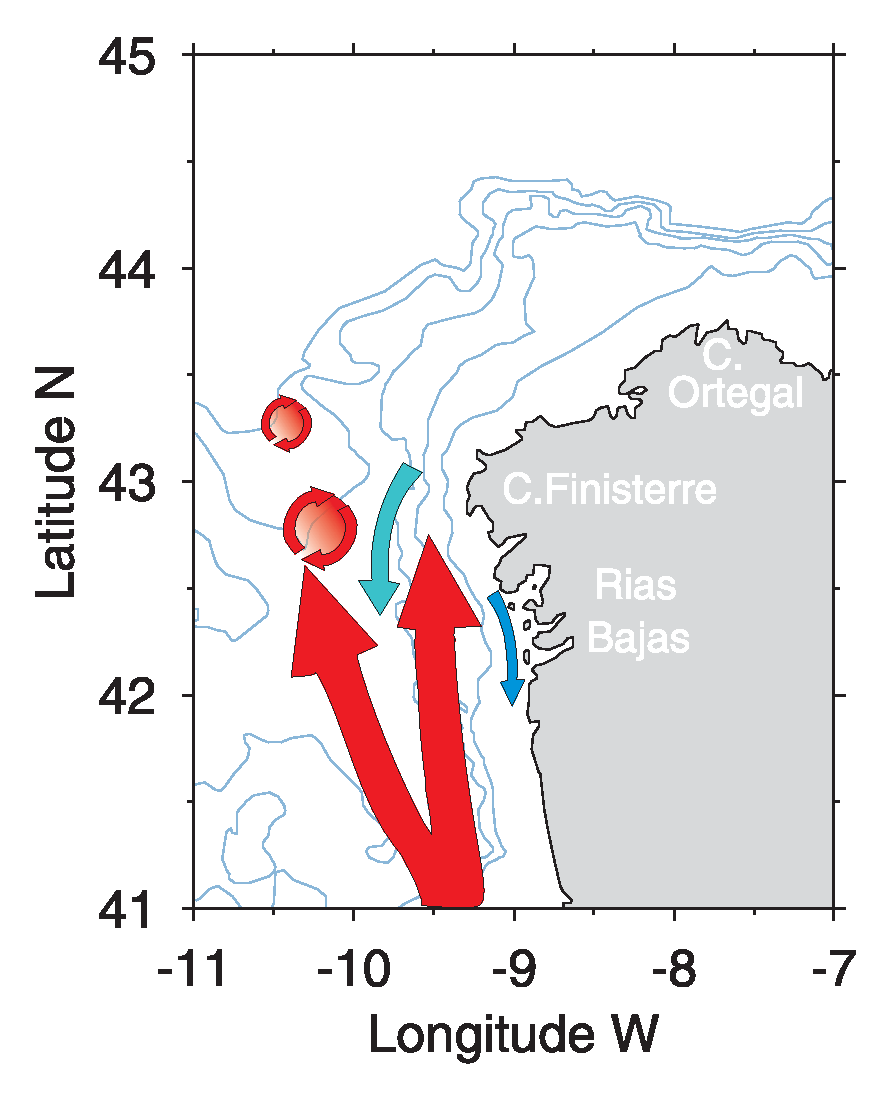
\includegraphics[width=7cm]{springcirc}}
\subfigure[]{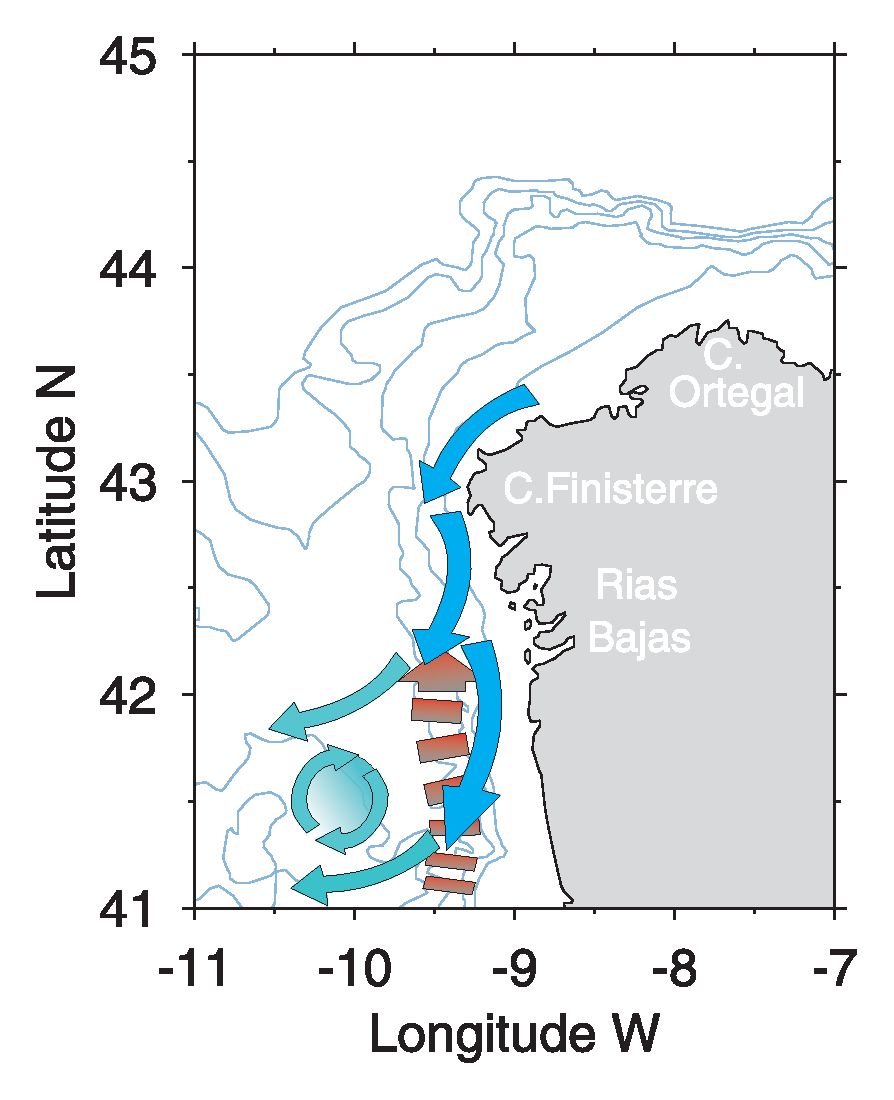
\includegraphics[width=7cm]{summercirc}}%
\subfigure[]{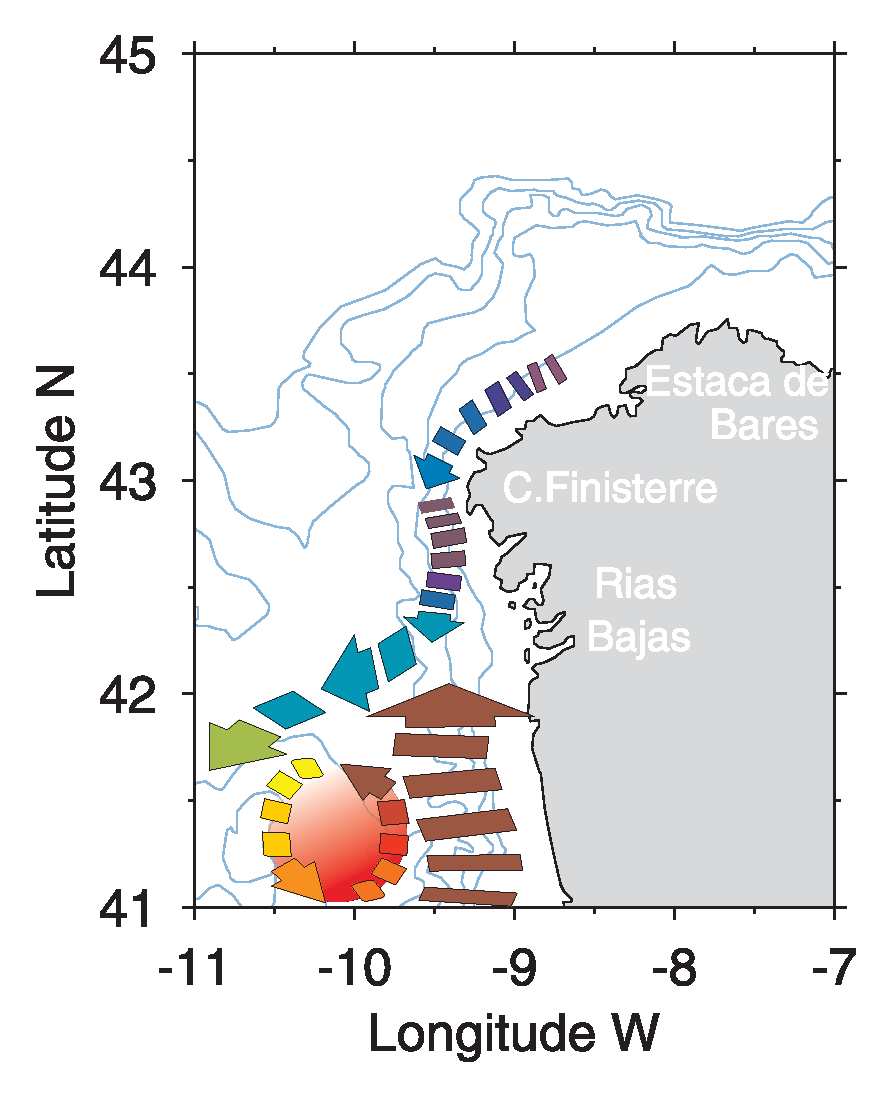
\includegraphics[width=7cm]{autumncirc}}
\caption{Schematic of the surface and subsurface circulation
during (a) winter, (b) spring, (c) summer and (d) autumn. A colour
scheme is used were red corresponds to warmer temperatures and
green/blue to cooler ones. See text for details }
\label{fig:concl_sketch}
\end{figure}

\subsection{The transition between downwelling to upwelling regime}
The weakening of the meridional density gradients sparks the decay
phase of the poleward slope current. The warm tongue has by now
broadened, and distorted by interactions with the mesoscale eddy
field (Fig~\ref{fig:concl_sketch}b). Upwelling favourable winds
push the flow offshore establishing a second northward flow
offshore, and eddies and upwelling dynamics break the slope flow
structure.
\subsection{The upwelling regime}
Upper column structure become dominated by upwelling and filaments
and poleward flow is restricted to deeper levels. Intensified flow
at Cape Finisterre from buoy measurements in all seasons for which
there was data. Cape induced upwelling maxima \citep{Rosenfeld94}

Interannual variability during the upwelling regime is
characterise by either presence/absence of filaments or whether
the main filament is at Cape Finisterre or at 42\deg latitude.

We managed to sample a filament, which in the light of the data
presented here, it is remarkable in itself as they have proved
very intermittent in recent years. This, in turn, supports the
idea of growing instabilities. An eddy field would generate
filaments whenever an upwelling front is present. As it is, only
when the upwelling is mature enough do filaments develop. However
the filament presented a very shallow structure which could only
be representative of a decaying structure or typical of the
Galician upwelling regime.

Differences between the 42\deg and Cape Finisterre Filament in
terms of forcing, persistence? and size/consequences.

\subsection{The transition between upwelling to downwelling
regime}
Weakening upwelling winds allows the poleward flow to climb back
onto the upper slope but is not until the meridional density
strengthens and upwelling winds weakens that the poleward flow
surfaces again.

\section{Future work}
Although there have been various significant efforts to observe
facets of the Galician or Iberian upwelling over the years e.g.
recently MORENA, OMEX II, there has never been a systematic effort
to monitor its year-round physical development with simultaneous
hydrographic, current and meteorological observations on the scale
of the California Current programs like CUEA or CODE. The
gradualist approach, while it has illuminated many aspects of the
system, has left many basic questions like the 3-d structure, the
spin up and spin down of upwelling, the importance of alongshore
propagating upwelling signals, unanswered.

Unresolved questions that need tackling are:

Coastal Trapped Waves (CTW) role in the system's evolution and
other high frequency sub-inertial signals. CTW could be of
importance given the large wind variability. \citet{Huthnance02}
reported that 4-6 day wind stress fluctuations excited a
second-mode CTW with 4-6 day current fluctuations which
corresponded to a phase speed of 2.2\vel. Similarly, inertial
waves could represent a quantifiable part of the observed
variability of the region.

Further detailed sampling of the 3-D filament structure are needed
in order to provide a more accurate description of its dynamics
and assess the relevance of the results presented here.

poleward tendency during summer and effect of north/west coast
upwelling in system evolution

A more intensive study of the poleward flow interannual
variability should unequivocally show the main source of the
variability and quantify the effect of the wind forcing in
precluding its year around presence.

upwelling undercurrent

smaller scale shelf circulation?

Large scale wind curl similar to Oregon coast and possible
poleward flow tendency.



Take ideas from COUPLE proposal.

Operational oceanography will be required of such a busy region
and data are needed to validate models and design measurement
networks to maximise resources.

Many of these questions could partially be tackled from a
modelling point of view. So far, existing modelling efforts have
been restricted to climatological experiments. Needs better and
more realistic topography, coast and wind forcing.
